% Options for packages loaded elsewhere
\PassOptionsToPackage{unicode}{hyperref}
\PassOptionsToPackage{hyphens}{url}
\PassOptionsToPackage{dvipsnames,svgnames,x11names}{xcolor}
\documentclass[
  10pt,
]{article}
\usepackage{xcolor}
\usepackage[margin=16mm]{geometry}
\usepackage{amsmath,amssymb}
\setcounter{secnumdepth}{-\maxdimen} % remove section numbering
\usepackage{iftex}
\ifPDFTeX
  \usepackage[T1]{fontenc}
  \usepackage[utf8]{inputenc}
  \usepackage{textcomp} % provide euro and other symbols
\else % if luatex or xetex
  \usepackage{unicode-math} % this also loads fontspec
  \defaultfontfeatures{Scale=MatchLowercase}
  \defaultfontfeatures[\rmfamily]{Ligatures=TeX,Scale=1}
\fi
\usepackage{lmodern}
\ifPDFTeX\else
  % xetex/luatex font selection
\fi
% Use upquote if available, for straight quotes in verbatim environments
\IfFileExists{upquote.sty}{\usepackage{upquote}}{}
\IfFileExists{microtype.sty}{% use microtype if available
  \usepackage[]{microtype}
  \UseMicrotypeSet[protrusion]{basicmath} % disable protrusion for tt fonts
}{}
\makeatletter
\@ifundefined{KOMAClassName}{% if non-KOMA class
  \IfFileExists{parskip.sty}{%
    \usepackage{parskip}
  }{% else
    \setlength{\parindent}{0pt}
    \setlength{\parskip}{6pt plus 2pt minus 1pt}}
}{% if KOMA class
  \KOMAoptions{parskip=half}}
\makeatother
\usepackage{longtable,booktabs,array}
\newcounter{none} % for unnumbered tables
\usepackage{calc} % for calculating minipage widths
% Correct order of tables after \paragraph or \subparagraph
\usepackage{etoolbox}
\makeatletter
\patchcmd\longtable{\par}{\if@noskipsec\mbox{}\fi\par}{}{}
\makeatother
% Allow footnotes in longtable head/foot
\IfFileExists{footnotehyper.sty}{\usepackage{footnotehyper}}{\usepackage{footnote}}
\makesavenoteenv{longtable}
\usepackage{graphicx}
\makeatletter
\newsavebox\pandoc@box
\newcommand*\pandocbounded[1]{% scales image to fit in text height/width
  \sbox\pandoc@box{#1}%
  \Gscale@div\@tempa{\textheight}{\dimexpr\ht\pandoc@box+\dp\pandoc@box\relax}%
  \Gscale@div\@tempb{\linewidth}{\wd\pandoc@box}%
  \ifdim\@tempb\p@<\@tempa\p@\let\@tempa\@tempb\fi% select the smaller of both
  \ifdim\@tempa\p@<\p@\scalebox{\@tempa}{\usebox\pandoc@box}%
  \else\usebox{\pandoc@box}%
  \fi%
}
% Set default figure placement to htbp
\def\fps@figure{htbp}
\makeatother
\setlength{\emergencystretch}{3em} % prevent overfull lines
\providecommand{\tightlist}{%
  \setlength{\itemsep}{0pt}\setlength{\parskip}{0pt}}
\usepackage{bookmark}
\IfFileExists{xurl.sty}{\usepackage{xurl}}{} % add URL line breaks if available
\urlstyle{same}
\hypersetup{
  colorlinks=true,
  linkcolor={Maroon},
  filecolor={Maroon},
  citecolor={Blue},
  urlcolor={Blue},
  pdfcreator={LaTeX via pandoc}}

\author{}
\date{}

\begin{document}

\section{Handout: Dual Geometry of Wavelength Space and Frequency Space
--- All 16 Papers + Survey (v2, fully published
2026-06-12)}\label{handout-dual-geometry-of-wavelength-space-and-frequency-space-all-16-papers-survey-v2-fully-published-2026-06-12}

\textbf{Noriaki Kihara (WF System Co., Ltd.~/ ORCID:
0009-0004-6753-4020) · CC BY 4.0}

\subsection{In one page}\label{in-one-page}

Three assumptions --- \textbf{νλ=1 (one relation), the zero point ½ (one
constant), one asymmetric bit} --- plus two operating principles
(configuration reading; the record principle). From this inventory
alone, the series tests how far quantum-looking and spacetime-looking
structures follow \textbf{as theorems}, in a discrete system that is
machine-checkable at every step. Sixteen papers plus a survey, bilingual
Japanese/English, published on Zenodo. \textbf{No physical
identification is made} (the central thesis: a different map with the
same results).

\subsection{Series map}\label{series-map}

{\def\LTcaptype{none} % do not increment counter
\begin{longtable}[]{@{}
  >{\raggedright\arraybackslash}p{(\linewidth - 4\tabcolsep) * \real{0.3333}}
  >{\raggedright\arraybackslash}p{(\linewidth - 4\tabcolsep) * \real{0.3333}}
  >{\raggedright\arraybackslash}p{(\linewidth - 4\tabcolsep) * \real{0.3333}}@{}}
\toprule\noalign{}
\begin{minipage}[b]{\linewidth}\raggedright
Part
\end{minipage} & \begin{minipage}[b]{\linewidth}\raggedright
Papers
\end{minipage} & \begin{minipage}[b]{\linewidth}\raggedright
Content
\end{minipage} \\
\midrule\noalign{}
\endhead
\bottomrule\noalign{}
\endlastfoot
Foundations & 1--4 & Lattice and counting: \(N_0\)(R)=1, 9, 137,
\ldots{} (pure enumeration); splitting; the hierarchical vacuum \\
Theorems & 5--12 & Dictionary theorem; freezing theorem (time's
condition = the one bit); exclusion as theorem; area law;
half-wavelength censorship; emergent gauge; \textbf{necessity of
dimension 4}; measurement = appending a record \\
Sequel & 13--16 & \textbf{Resolution of position and time}; time
direction = complex structure; constructed \& verified coordinate map;
\textbf{reduction of the measure problem} \\
Survey & --- & The dictionary to standard theory and the \textbf{axiom
exchange balance} \\
\end{longtable}
}

\subsection{Main results of the sequel (published
2026-06-12)}\label{main-results-of-the-sequel-published-2026-06-12}

\textbf{Paper 13 --- Position Had Never Been Read}: discrete position =
the wave's sign sector (zero additions to the state space). Space = the
Pontryagin dual of the conserved-quantity lattice (its three symmetries
are theorems of duality). Three readout strata \textbf{11⊂13⊂21}
(intensity-only fringes lose about half the information in principle).
Clock targets = \textbf{all odd integers --- proven via Gauss's
triangular-number theorem}. t is a derived quantity (no independent
inverse map).

\textbf{Paper 14 --- Time Direction and the Stage of Amplitudes}:
choosing a time direction = choosing a complex structure (exactly 16
lattice-compatible structures, a single \(B_4\) orbit). The transport
phase is derived and lands in \textbf{\(Z_4\) without exception}.
Symmetrization postulate → \textbf{canonical-convention theorem} (a
consequence of set structure).

\textbf{Paper 15 --- Projection onto xyztRQ}: explicit forward and
inverse maps, state → (x,y,z,t,R,Q), built as a five-stage operation;
\textbf{round trip 500/500; commutes with the conservation laws}
(charge-like parity = a theorem of support arithmetic: 39.2\% of raw
combinations are violation candidates, yet zero violations among
contributing paths). Velocity exists only in the sequence of records.

\textbf{Paper 16 --- The Rigorous Reduction of the Measure Problem}:
\textbf{no aggregation rule is selected.} The historical proximity
0.0007 = an artifact of two-outcome compression (with three outcomes the
divergence jumps three orders). Interference granularity is not a
convention: the mirror parent yields \textbf{W=0 (exact) ∧ W′=768
(exact)}. The remaining freedom reduces to \textbf{granularity × one
event bit × conditioning}, with a table of adjudication experiments
installed inside the model. The Born rule = ``an effective law to merge
with in the appropriate limit'' (triple criterion: convergence,
suppression, prediction).

\begin{figure}
\centering
\pandocbounded{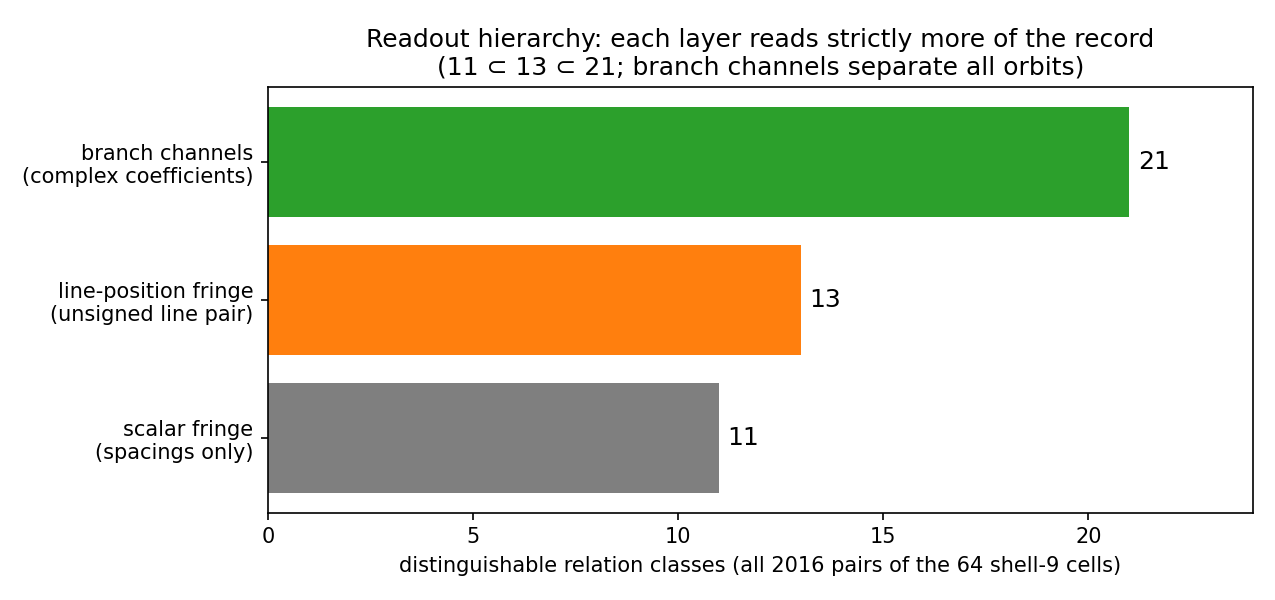
\includegraphics[keepaspectratio,alt={The readout hierarchy 11 in 13 in 21}]{paper13_fig2_readout_layers.png}}
\caption{The readout hierarchy 11 in 13 in 21}
\end{figure}

\begin{figure}
\centering
\pandocbounded{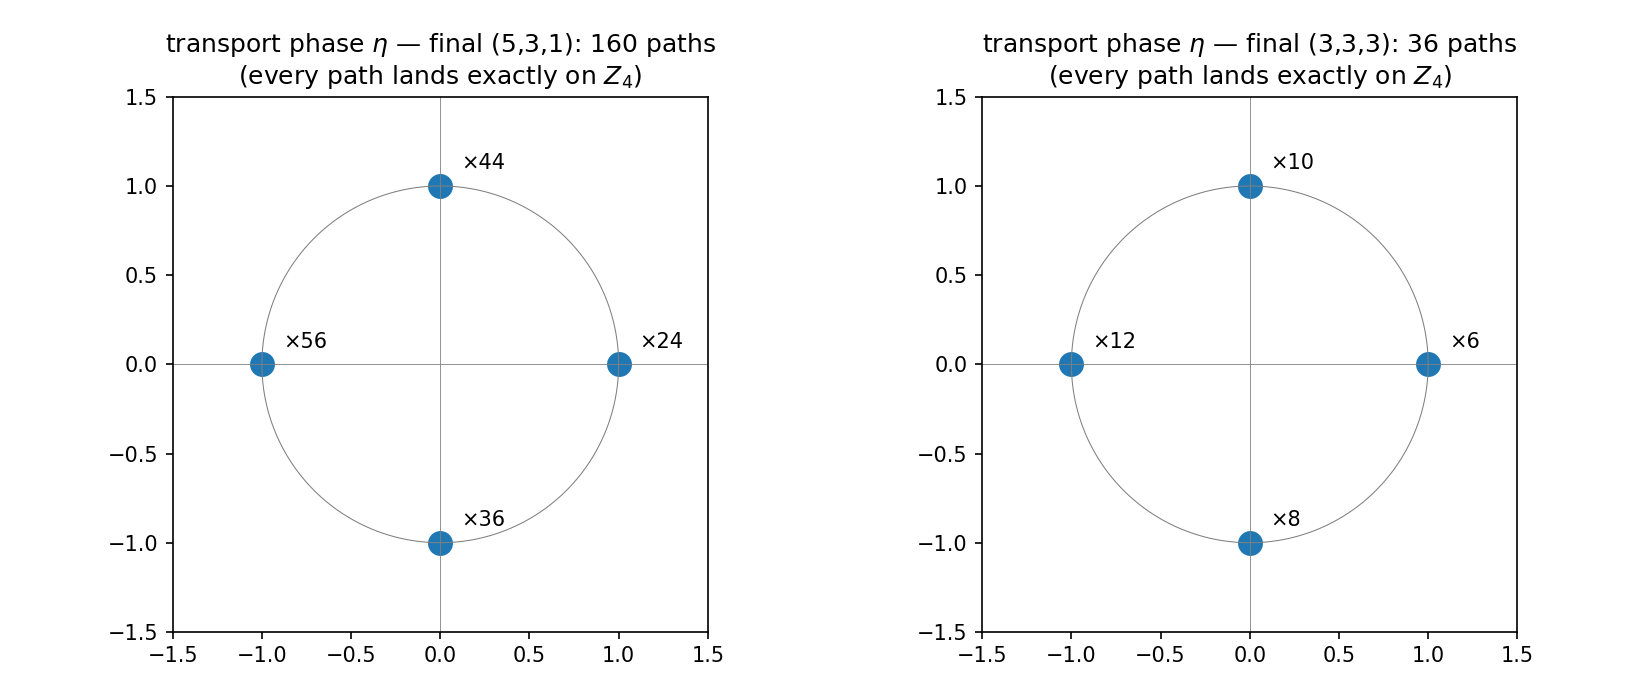
\includegraphics[keepaspectratio,alt={Transport phases land exactly on Z4}]{paper14_fig1_eta_z4.png}}
\caption{Transport phases land exactly on Z4}
\end{figure}

\begin{figure}
\centering
\pandocbounded{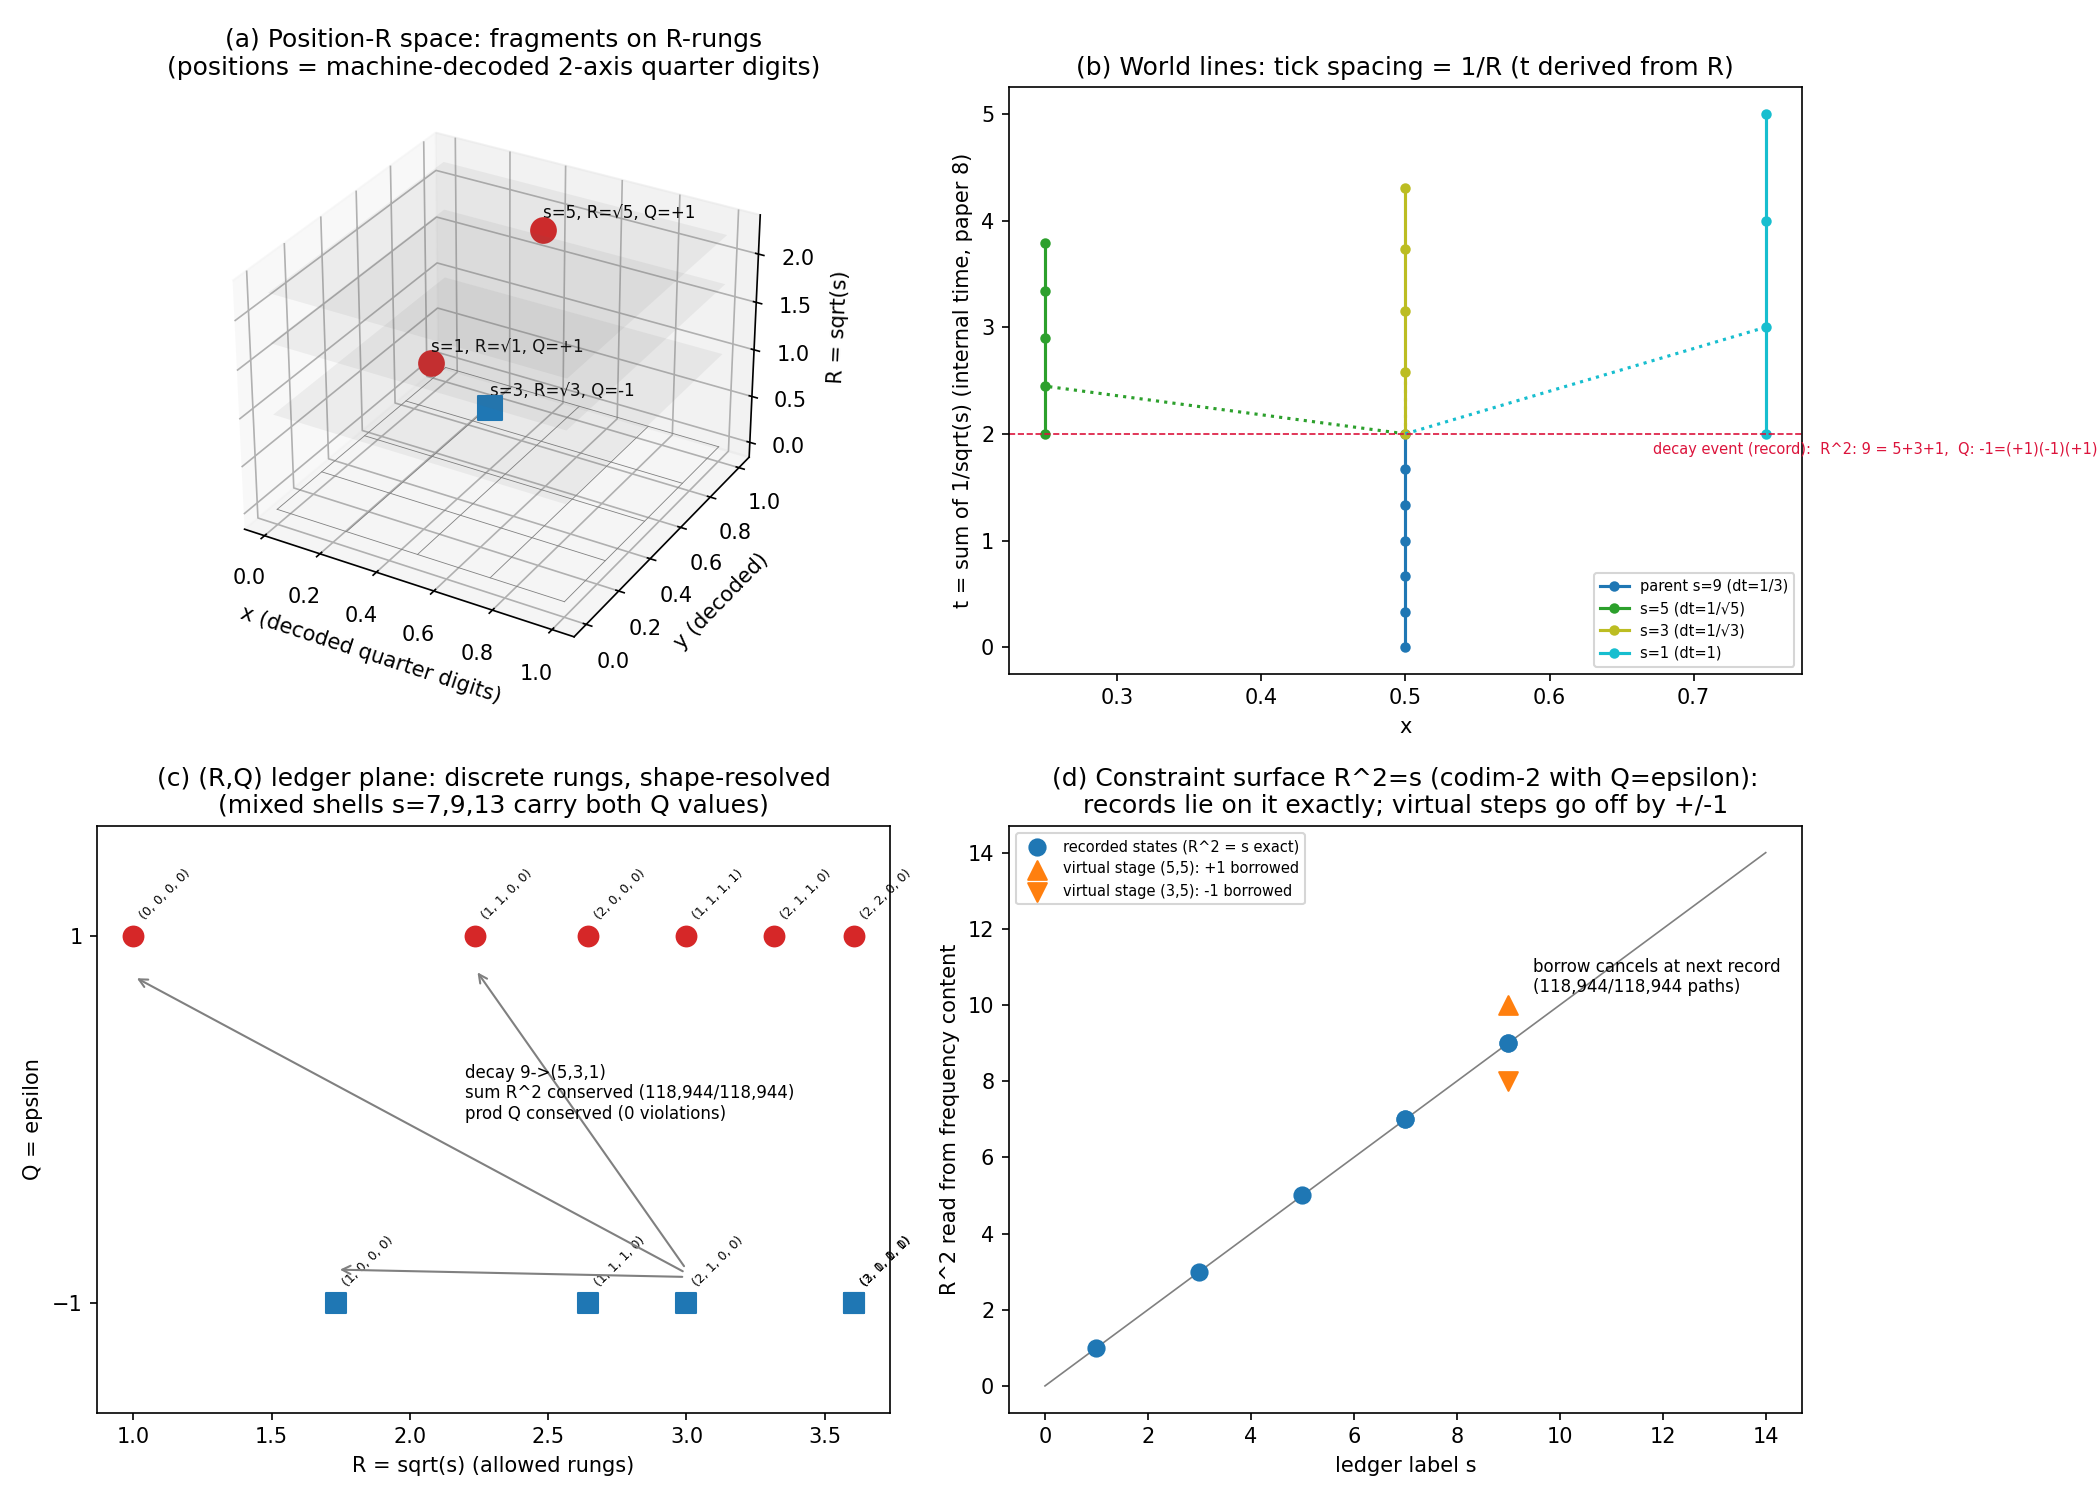
\includegraphics[keepaspectratio,alt={The xyztRQ space at a glance}]{paper15_fig2_xyztRQ.png}}
\caption{The xyztRQ space at a glance}
\end{figure}

\begin{figure}
\centering
\pandocbounded{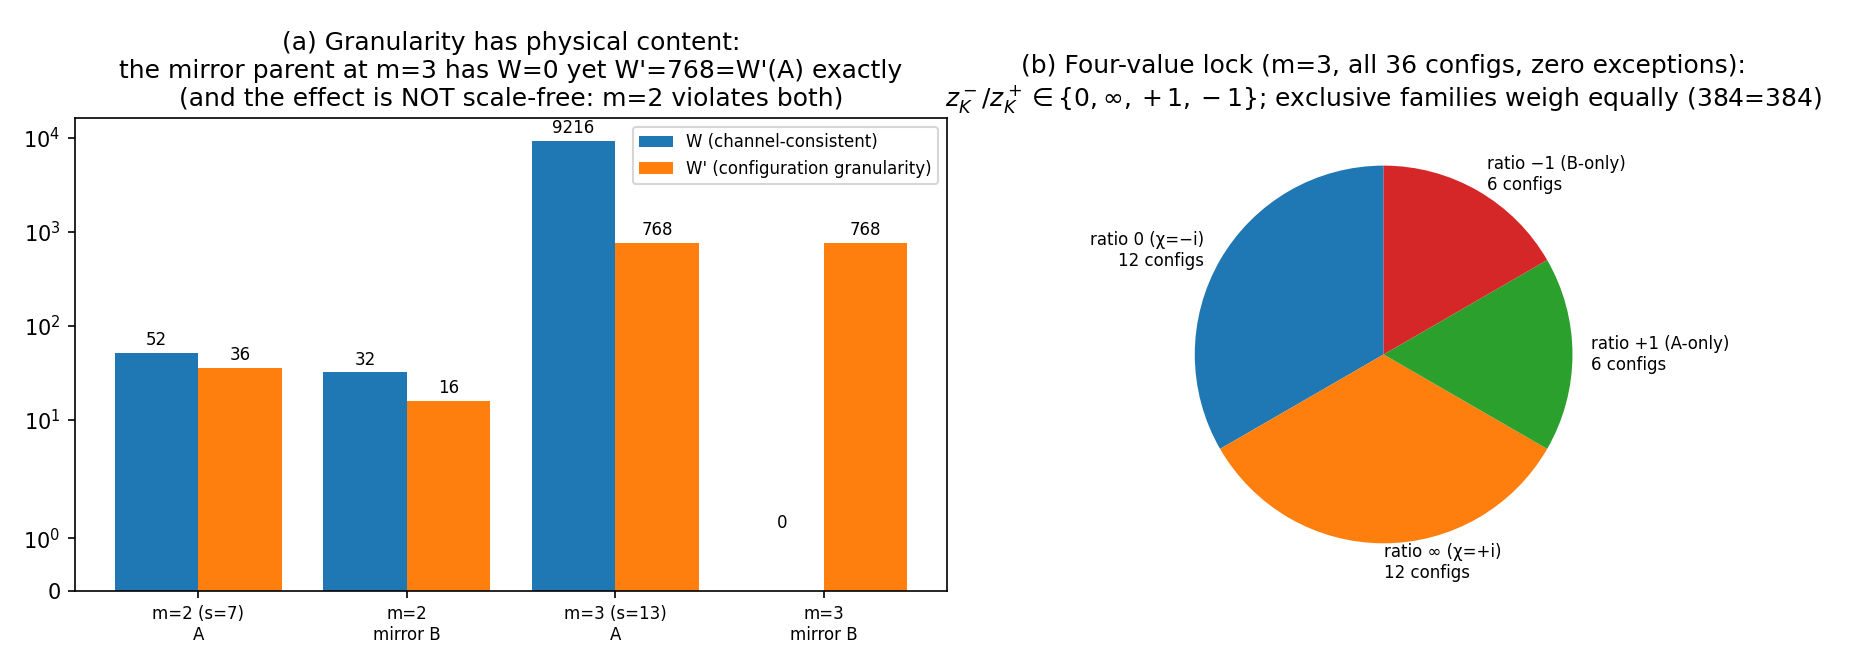
\includegraphics[keepaspectratio,alt={Granularity is not a convention; the four-value lock}]{paper16_fig3_granularity.png}}
\caption{Granularity is not a convention; the four-value lock}
\end{figure}

▲ Top to bottom: the readout hierarchy (intensity 11 ⊂ line-position 13
⊂ branch channels 21 = complete separation; Paper 13) / transport phases
landing on Z4 (all 196 paths, zero exceptions; Paper 14) / the mirror
cancellation W=0 with W'\textgreater0 and the four-value lock (Paper
16). All figures are exact computations.

\subsection{The survey: the axiom exchange
balance}\label{the-survey-the-axiom-exchange-balance}

{\def\LTcaptype{none} % do not increment counter
\begin{longtable}[]{@{}
  >{\raggedright\arraybackslash}p{(\linewidth - 4\tabcolsep) * \real{0.3333}}
  >{\raggedright\arraybackslash}p{(\linewidth - 4\tabcolsep) * \real{0.3333}}
  >{\raggedright\arraybackslash}p{(\linewidth - 4\tabcolsep) * \real{0.3333}}@{}}
\toprule\noalign{}
\begin{minipage}[b]{\linewidth}\raggedright
Axiom in standard theory
\end{minipage} & \begin{minipage}[b]{\linewidth}\raggedright
In this system
\end{minipage} & \begin{minipage}[b]{\linewidth}\raggedright
Source
\end{minipage} \\
\midrule\noalign{}
\endhead
\bottomrule\noalign{}
\endlastfoot
Symmetrization postulate & \textbf{Theorem} (canonical convention) &
Paper 14 \\
Time = external parameter & \textbf{Theorem} (derived quantity) & Papers
13, 15 \\
Measurement postulate & \textbf{Theorem} (appending + record) & Paper
12 \\
Spacetime dimension = input & \textbf{Theorem} (necessity) & Paper 11 \\
Charge conservation & \textbf{Theorem} (support parity arithmetic) &
Paper 15 \\
\end{longtable}
}

Payment: one relation + one constant + one bit + two operating
principles. \textbf{Only two entries remain blank: measure and action.}
Thesis: a completely filled dictionary = re-notation = zero empirical
content. \textbf{The incomplete points of the connection are the only
places where observation can adjudicate} --- the remainder is at once a
deficiency and a map of decidability.

\subsection{Verification regime}\label{verification-regime}

Every claim is supported by exhaustive verification, exact identities,
and machine-precision numerics; all figures are exact computations (no
schematics). Papers 13--16 passed a \textbf{two-party AI
independent-verification protocol} (local machine verification ×
independent re-computation and review): \textbf{two rounds each, eight
reviews in total}, with seven mutual corrections (including refuted
predictions and retractions) --- \textbf{the history is published
undeleted}.

\subsection{Access}\label{access}

\begin{itemize}
\tightlist
\item
  \textbf{Papers 1--16}: Zenodo Concept DOIs 10.5281/zenodo.20588036 --
  20665699 (full list in 論文一覧.md)
\item
  \textbf{Survey}: 10.5281/zenodo.20666132
\item
  \textbf{Repository snapshot} (permanent archive of everything):
  10.5281/zenodo.20666114
\item
  \textbf{Repository} (84 supplements, all scripts, review records,
  indexes): https://github.com/WurabeSeiji/ai-chat-logs-open (folder:
  波長空間と周波数空間の双対幾何)
\end{itemize}

\subsection{Standing (restated)}\label{standing-restated}

Not an attempt at a new or unified theory. \textbf{``Structures close to
standard quantum theory may be derivable from a different set of simple
assumptions''} --- that is the prescribed reading. \(N_0\)(3)=137 is not
identified with the fine-structure constant. No measure has been
selected. Numerical conversion to physical units would require an
independent dimensionless observable (stated as unresolved).

\end{document}
